\subsection{Preventivo a Finire}\label{caption_paf}

Nella seguente sezione inseriremo il preventivo a finire. Qualora non fosse presente il consuntivo di fine periodo utilizzeremo il preventivo. \\

\begin{longtable}{| C{.30\textwidth}| C{.15\textwidth}| C{.20\textwidth}|}
\hline
\rowcolor{bluelogo}\textbf{\textcolor{white}{Periodo}} & \textbf{\textcolor{white}{Preventivo in \euro}} & \textbf{\textcolor{white}{Consuntivo in \euro}} \\
\hline
Avvio ed Analisi dei Requisiti & \EUR{3870.00} & \EUR{4005.00} \\
\hline
\rowcolor{grigio}Risanamento Criticità & \EUR{775.00}  & \EUR{490.00} \\
\hline
Progettazione Architetturale & \EUR{3127.00} & \EUR{3183.00} \\
\hline
\rowcolor{grigio} Risanamento Criticità & \EUR{426.00} & \EUR{426.00} \\
\hline
Progettazione di Dettaglio e Codifica & \EUR{6669.00} & \EUR{6464.00} \\
\hline
\rowcolor{grigio} Risanamento Criticità &  \EUR{426.00} & \EUR{526.00} \\
\hline
Validazione e Collaudo & \EUR{2620.00}  & \EUR{2448.00} \\
\hline
\rowcolor{grigio}\textbf{Totale} & \EUR{14043.00}  & \textbf{\EUR{13537.00}}  \\
\hline
\caption{Preventivo a Finire}
\label{paf}
\end{longtable}

\subsubsection{Conclusioni}\label{PAF_RA}
Il costo finale del prodotto si attesta, quindi, ad \EUR{13537.00}, con una riduzione di \EUR{506.00} rispetto a quanto inizialmente preventivato. Tale differenza è dovuta principalmente a causa di un apporto lavorativo inferiore rispetto a quello preventivato da parte di un membro del gruppo. 

\begin{longtable}{|C{.30\textwidth}|C{.06\textwidth}|C{.06\textwidth}|C{.06\textwidth} | C{.06\textwidth}| C{.06\textwidth} | C{.06\textwidth} | C{.10\textwidth} |}
	\hline
	\rowcolor{bluelogo}	\textbf{\textcolor{white}{Nome}} & \textbf{\textcolor{white}{RE}} & \textbf{\textcolor{white}{AM}} & \textbf{\textcolor{white}{AN}} & \textbf{\textcolor{white}{PJ}} & \textbf{\textcolor{white}{PR}} & \textbf{\textcolor{white}{VE}} & \textbf{\textcolor{white}{Totale}}\\
	\hline \hline
	
	Marco Chilese & 8 & 12 & 5 & 35 & 13 & 32 & 105\\
	\hline
	\rowcolor{grigio}Marco Favaro & 8 & 10 & 22 & 14 & 19 & 32 & 105 \\
	\hline
	Diego Mazzalovo & 6 & 8 & 4 & 38 & 26  & 23 & 105\\
	\hline
	\rowcolor{grigio}Carlotta Segna & 0 & 18 & 15 & 10 & 46 & 16 & 105\\
	\hline
	Matteo Slanzi & 8 & 0 & 2 & 21 & 24 & 32 & 87\\
	\hline
	\rowcolor{grigio}Bogdan Stanciu & 7 & 11 & 8 & 21 & 35 & 23 & 105 \\
	\hline
	Luca Violato & 9 & 8 & 14 & 22 & 28 & 24 & 105\\
	\hline
	\rowcolor{grigio}\textbf{TOT} & 46 & 67 & 70 & 161 & 191 & 182 & 717\\
	\hline
	\caption{Distribuzione oraria totale per ruolo per persona}
	\label{orePersona}
\end{longtable}

\begin{center}
	\begin{figure}[H]
		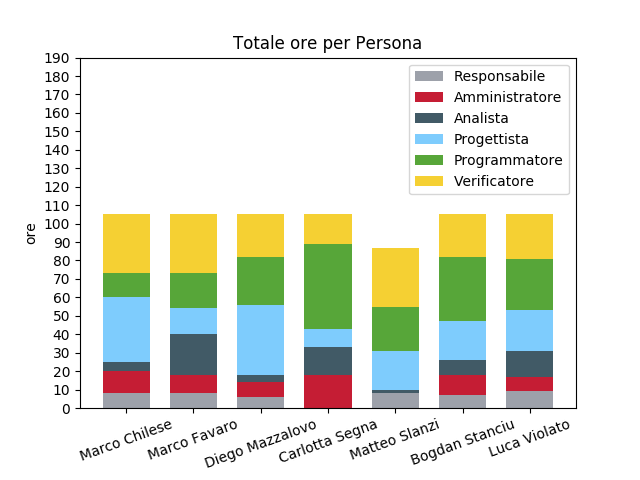
\includegraphics[scale=0.9]{./images/totPersonaOre.png}
		\caption{Totale ore Rendicontate per Persona}
	\end{figure}
	\begin{figure}[H]
		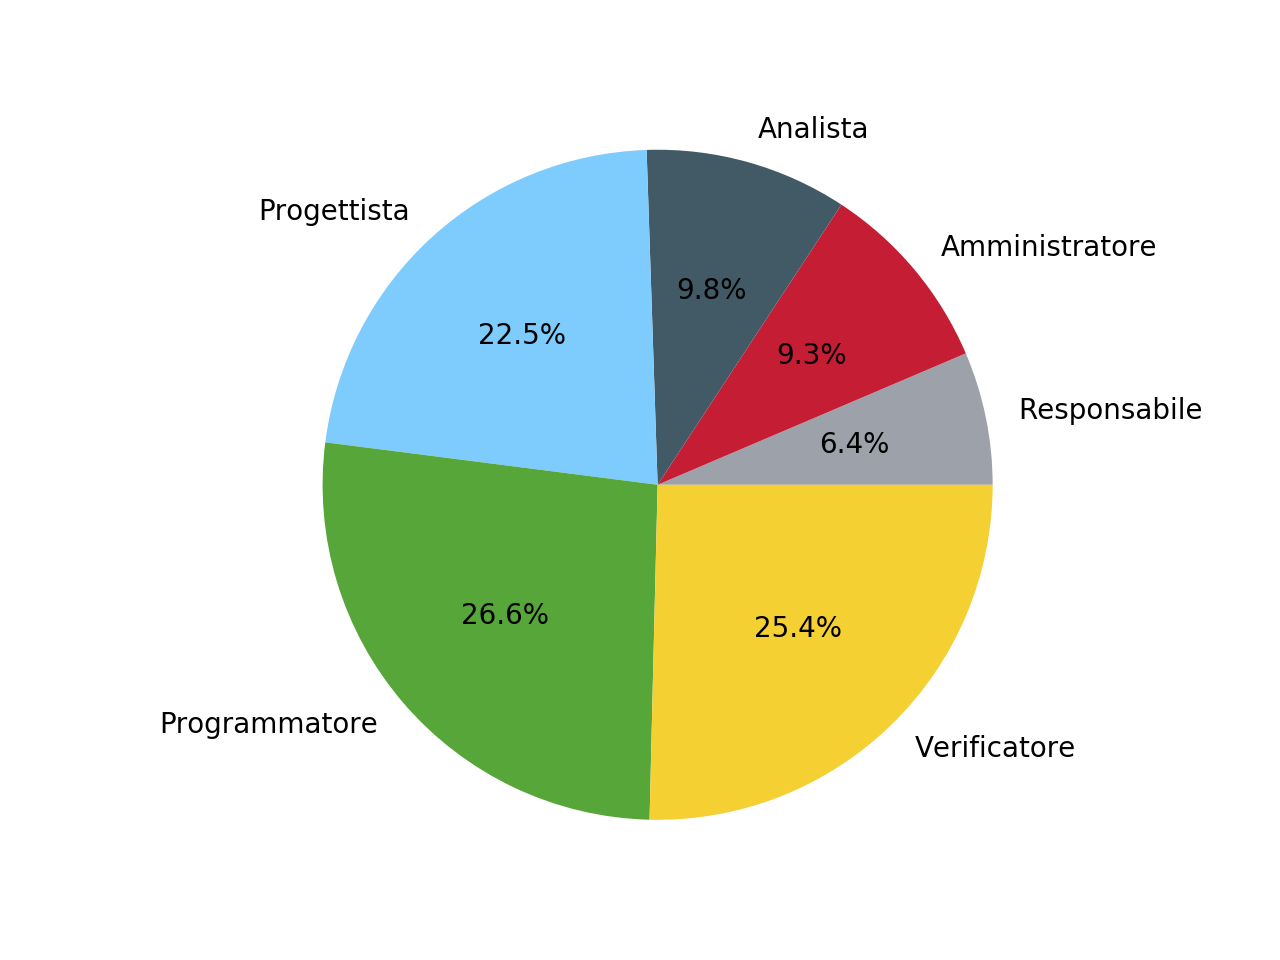
\includegraphics[scale=0.7]{./images/torta_totPersonaOre.png}
		\caption{Totale ore Rendicontate per Ruolo}
	\end{figure}
\end{center}

\newpage
